\section{eplusout.dxf}\label{eplusout.dxf}

The DXF output report file is formatted according to the ``Data Exchange Format'' standard rules for representing CADD type coordinates. The file can be used in several inexpensive, shareware or freeware viewers. Quickview Plus\textsuperscript{TM} can display DXF files as shown in Figure~\ref{fig:quick-view-plus-version-of-dxf-file} below. A free program originally from Autocad\textsuperscript{TM}, Voloview Express\textsuperscript{TM}, can display solid model rendering as shown in Figure~\ref{fig:voloview-3d-solid-view}. Other viewers are available from Microstation\textsuperscript{TM}, Visio\textsuperscript{TM} and other shareware or freeware vendors.

This file is generated when the following line is included in the IDF.

\textbf{Output:Surfaces:Drawing, DXF;}

You can ask it to triangulate surfaces with \textgreater{}4 sides:

\textbf{Output:Surfaces:Drawing, DXF, Triangulate3dface;}

In addition to the building shape (including detached shading elements), the DXF view includes a ``true north'' arrow (at ground level) and the name from the BUILDING object.

\begin{figure}[hbtp] % fig 1
\centering
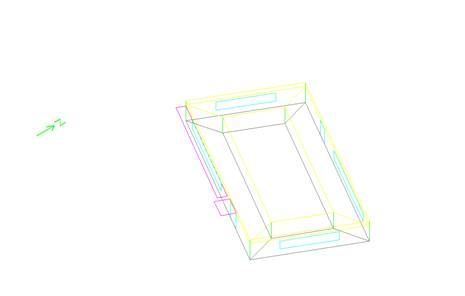
\includegraphics[width=0.9\textwidth, height=0.9\textheight, keepaspectratio=true]{media/image001.jpg}
\caption{Quick View Plus version of DXF file \protect \label{fig:quick-view-plus-version-of-dxf-file}}
\end{figure}

Even in the Quick View version, you can see that the different building elements have different colors. These are the ``original'' colors used in EnergyPlus. The current default color scheme is shown in the following figure of the solid model.

\begin{figure}[hbtp] % fig 2
\centering
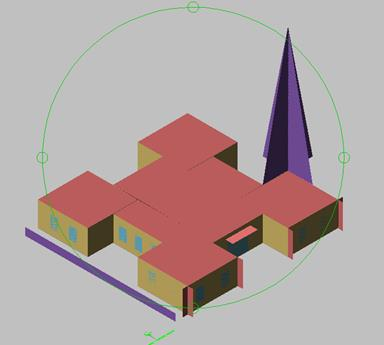
\includegraphics[width=0.9\textwidth, height=0.9\textheight, keepaspectratio=true]{media/image002.jpg}
\caption{Voloview 3D Solid view \protect \label{fig:voloview-3d-solid-view}}
\end{figure}

The DXF file of itself is an ASCII file, with a specific structure as specified in the standard. An excerpt of the file is shown below:

\begin{lstlisting}
SECTION
  2
ENTITIES
  0
TEXT
  8
1
  6
CONTINUOUS
 62
  3
 10
      -11.00000
 20
        3.00000
 30
        0.10000
 40
 .25
  1
True North
 41
 0.0
  7
MONOTXT
210
0.0
220
0.0
230
1.0
  0
\end{lstlisting}

\begin{lstlisting}
3DFACE
  8
1
 62
  3
 10
      -10.00000
 20
        3.00000
 30
        0.10000
 11
      -10.00000
 21
        3.00000
 31
        0.00000
 12
      -10.00000
 22
        0.00000
 32
        0.00000
 13
      -10.00000
 23
        0.00000
 33
        0.10000
  0
ENDSEC
  0
EOF
999
DXF created from EnergyPlus
999
\end{lstlisting}

Program Version,EnergyPlus, \textless{}version\textgreater{}
